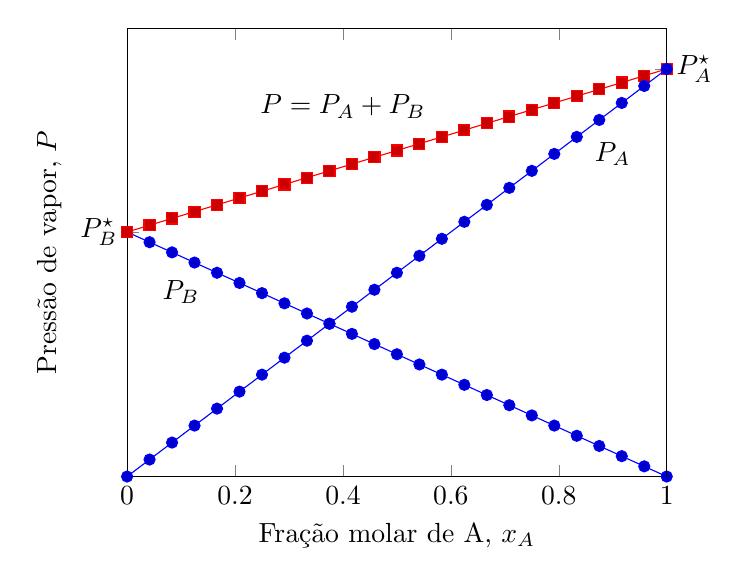
\begin{tikzpicture}
    \begin{axis}
        [
            grid = minor,
            axis y line* = left,
            xlabel = {Fração molar de \ce{A}, $x_{\ce{A}}$},
            ylabel = {Pressão de vapor, $P$},
            xmin = 0, xmax = 1,
            ymin = 0, ymax = 55,
            ytick = {30},
            yticklabels = {$P_{\ce{B}}^\star$},
        ]     
        \addplot+ [domain = 0:1]
            { 
                30*(1 - x)
            };
            
        \addplot+ [red, domain = 0:1]
            { 
                30*(1 - x) + 50*x
            };
            
        \node [anchor = south] at (axis cs:0.1, 20) 
                { $P_{\ce{B}}$ };
    
        \node [anchor = north] at (axis cs:0.4, 48) 
                { $P = P_{\ce{A}} + P_{\ce{B}}$ };
    \end{axis}
    \begin{axis}
        [
            grid = minor,
            axis y line* = right,
            hide x axis,
            xmin = 0, xmax = 1,
            ymin = 0, ymax = 55,
            ytick = {50},
            yticklabels = {$P_{\ce{A}}^\star$},
        ]
        \addplot+ [domain = 0:1]
            { 
                50*x
            };
    
        \node [anchor = south] at (axis cs:0.9, 37) 
                { $P_{\ce{A}}$ };
    \end{axis}
    \end{tikzpicture}